%Latex Templates, Lab report for Universidad Tecnologica de Pereira
%Physics I,II,III Lab.
%feedback:hfjimenez@utp.edu.co 
\documentclass{article}
\usepackage[utf8]{inputenc}							%Tildes
\usepackage{gensymb}								% Generic symbols for both text and math mode
\usepackage{graphicx}								%Graficas, rapiditas.
 \usepackage{booktabs}
 \usepackage{multirow}
 \usepackage{subcaption}							
 \usepackage{float}									% Image will be in the same place as you want.!!! x-/

\title{Laboratorio 4. Ondas Estacionarias En Un Tubo Abierto Y Tubo Cerrado}
\author{Carlos Alberto Dagua Conda, Héctor Fabio Jiménez Saldarriaga, \\Juan Camilo Castrillon,\thanks{carlosdaguaco@utp.edu.co, hfjimenez@utp.edu.co, jucacastrillon@utp.edu.co} }
\date{Abril 2016}
\begin{document}
\maketitle
\section{Abstract}
In this paper we study experimentally the standing wave patterns and associated mathematics for closed-end air column using instrument consisting of a closed-end column typically containing a plastic tube in which one of the ends is covered and not open to the surrounding air. We use a 90cm plastic tube and transformed it into open-end air columns and a 50cm plastic tube close-end air by covering the end opposite the mouthpiece with a mute. We anal. We analyze the presence of the closed end on such an air column will affect the actual frequencies that the instrument were producing.

\section{Introducción}
\textbf{Objetivos}
\begin{itemize}
\item Identificar los distintos modos de vibración de las columnas de aire en uno tubo abierto y cerrado.
\item Medir la velocidad del sonido en el aire.
\end{itemize}
Las ondas estacionarias en una columna de aire presentes en un tubo, se generan por la superposición de ondas incidentes y reflejadas en el interior del mismo en estado de resonancia esto afectado también en sí el tubo es abierto o cerrado. Pero a diferencia de los modos propios de oscilación en una cuerda, en una columna de aire, estos no se pueden ver a simple vista; para ello se hacen uso de herramientas físicas para por medio de frecuencia y periodo calcular su modo de vibración para ello se contemplan los fenómenos presentes en las ondas de presión (rarefacción y compresión) y en las ondas de desplazamiento.
$$\\$$
\textbf{Tubos Abiertos}\newline
En \textbf{X = 0} y \textbf{ x = L}, las moléculas de aire tienen un valor máximo de desplazamiento a partir de su posición de equilibrio, definiendo un tubo abierto en ambos extremos.Las frecuencias de resonancia correspondientes a los distintos modos propios de oscilación de la columna de aire en un tubo abierto están dadas por:

Donde v es la velocidad del sonido en el aire. 
\begin{equation}
{ f }_{ n }=\frac { n }{ 2*L } v,\quad n=1,2,3,...
\end{equation}
\begin{figure}[H]
  \centering
     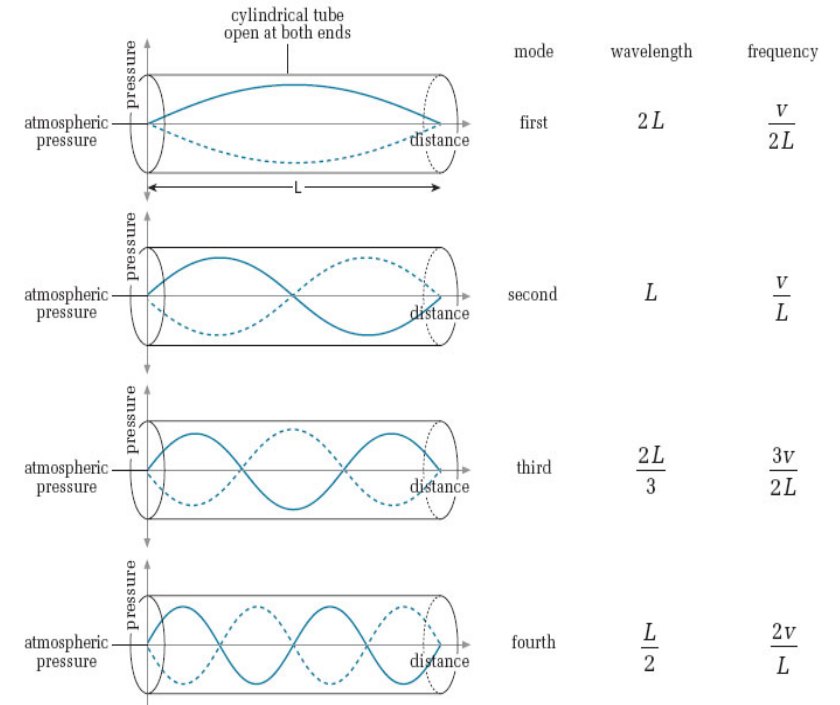
\includegraphics[width=0.85\textwidth]{p1}
  \caption{Patrones de ondas estacionarias correspondientes a ondas de presión en un tubo abierto en los dos extremos.}
      \label{fig:p1}
\end{figure}

La figura anterior, muestra el tono fundamental y algunos sobre tonos para la onda $\varphi $ de presión. Estos están desfasados $90^oC$ con las ondas de desplazamiento. Las frecuencias de resonancia ($f_{n}$) también se conocen con el nombre de armónicos.\newline
\textbf{Tubos Cerrados}\newline
En x = 0, la onda estacionaria tiene un valor máximo y en $\textbf{x = L}$ tiene un valor mínimo con respecto al desplazamiento de las moléculas de aire o a partir de la posición de equilibrio. Esto define un tubo cerrado.
Aplicando estas condiciones de frontera y llevando a cabo los cálculos apropiados, se encuentra que las frecuencias de resonancia en tubo cerrado están dadas por:
\begin{equation}
{ f }_{ n }=\frac { n }{ 4*L } v,\quad n=1,3,5,...
\end{equation}
\begin{figure}[H]
  \centering
     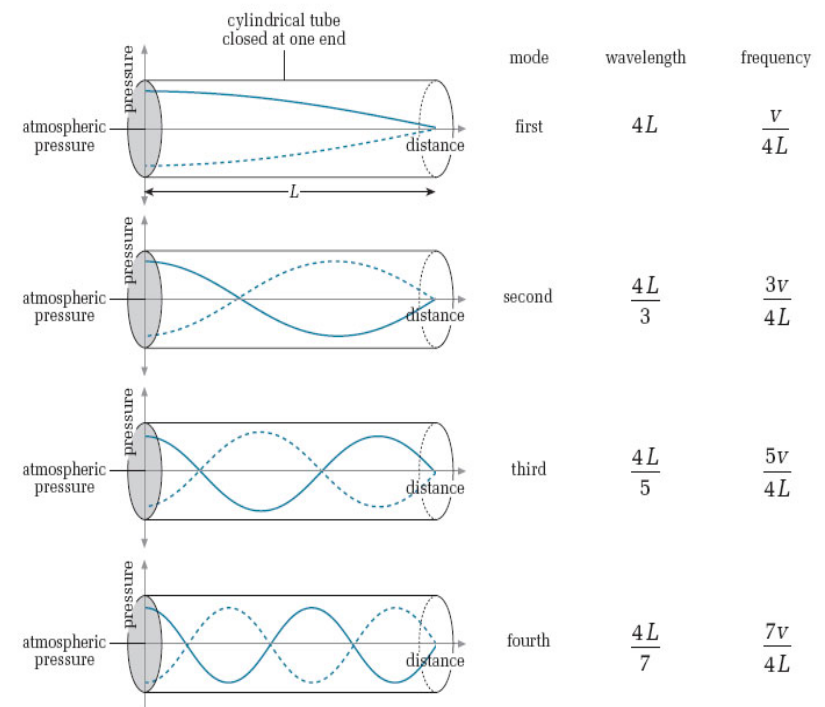
\includegraphics[width=0.85\textwidth]{p2}
  \caption{Patrones de ondas estacionarias correspondientes a ondas de presión en un tubo cerrado en un extremo y abierto en el otro.}
      \label{fig:p2}
\end{figure}
Las fórmulas y diagramas mostrados para resonancia en tubos son aproximadas, debido a que el comportamiento de las ondas en los extremos del tubo depende parcialmente de factores tales como el diámetro del tubo y la frecuencia de las ondas. Los extremos del tubo no son exactamente nodos o anti nodos. Las siguientes formulas empíricas deben utilizarse para la corrección de la longitud del tubo.
\begin{itemize}
\item Para un tubo abierto:
\begin{equation}
L^{'}=L+0.8d
\end{equation}
\item Para un tubo cerrado:
\begin{equation}
L^{'}=L+0.4d
\end{equation}
\end{itemize}
Para esta practica de Ondas Estacionarias En Un Tubo Abierto Y Tubo Cerrado 
\begin{table}[H]
\centering
\begin{tabular}{l|l|l|l|l|l|}
\cline{2-6}
                         & Periodo T & Frecuencia sin escala & Frecuencia {[}Hz{]} & $F_{i}$/ $F_{1}$  & Armónico n \\ \hline
\multicolumn{1}{|l|}{F1} & 5.4       & 0.18518               & 185.18              & 1     & 1          \\ \hline
\multicolumn{1}{|l|}{F2} & 2.8       & 0.35714               & 357.14              & 1.928 & 2          \\ \hline
\multicolumn{1}{|l|}{F3} & 1.7       & 0.5882                & 588.2               & 3.176 & 3          \\ \hline
\multicolumn{1}{|l|}{F4} & 1.3       & 0.76923               & 769.23              & 4.153 & 4          \\ \hline
\multicolumn{1}{|l|}{F5} & 1.2       & 0.90909               & 909.09              & 4.909 & 5          \\ \hline
\end{tabular}
\caption{Tabla 1. Medidas y análisis correspondientes en tubo abierto, $L=90cm$, $Temperatura=28^oC$}
\label{tabla1}
\end{table}
\begin{table}[h ]
\centering
\begin{tabular}{l|l|l|l|l|l|}
\cline{2-6}
                         & Periodo T & Frecuencia sin escala & Frecuencia {[}Hz{]} &  $F_{i}$/ $F_{1}$  & Armónico n \\ \hline
\multicolumn{1}{|l|}{F1} & 0.6       & 1.6666                & 166.6               & 1      & 1          \\ \hline
\multicolumn{1}{|l|}{F2} & 1.8       & 0.5555                & 555.5               & 3.334  & 3          \\ \hline
\multicolumn{1}{|l|}{F3} & 1.2       & 0.83333               & 833.3               & 5.001  & 5          \\ \hline
\multicolumn{1}{|l|}{F4} & 0.84      & 1.1904                & 1190.4              & 7.145  & 7          \\ \hline
\multicolumn{1}{|l|}{F5} & 0.7       & 1.4285                & 1428.5              & 8.5744 & 9          \\ \hline
\end{tabular}
\caption{Tabla 2. Medidas y análisis correspondientes en tubo cerrado, $L=50cm$, $Temperatura=28^oC$}
\label{tabla2}
\end{table}
\section{Análisis}
\subsection{(Pregunta 4.7.1)}
\textit{\textbf{1.} Para cada configuración del tubo (abierto y cerrado) divida cada una de las frecuencias de resonancia halladas por la frecuencia de resonancia más baja que encontró. Sus resultados deberían dar una serie de números cercanos a números enteros. ¿ Confirman sus resultados esta aseveración?. Explique.}
\newline
Para la tabla 1 correspondiente a un tubo abierto, tras dividir cada una de las frecuencias $F_{i}$ por la primera de las frecuencias$F_{1}$, obtuvimos un número muy aproximado a un entero. Este número n que obtuvimos en si el número del armónico el cual se explicó con anterioridad en el pre informe, para el caso de un tubo abierto este toma los armónicos $n={1,2,3,4,5}$
\newline
Para la tabla 2 correspondiente a un tubo cerrado, tras dividir cada una de las frecuencias  $F_{i}$ por la primera de las frecuencias $F_{1}$, obtuvimos un resultado similar al del tubo abierto, con la diferencia en la secuencia de dichos armónicos varían de tal forma que solo se toman los números impares $n= {1,3,5,7,9}$
\subsection{(Pregunta 4.7.2)}
\textit{\textbf{2.} ¿ Es la serie de números que usted ha hallado, la misma para tubo cerrado que para tubo abierto?.}
\newline
Al comparar el resultado de los armónicos n en cada una de las tablas se puede observar que aunque el primer armónico F1 es igual en cada tabla, conforme se avanza en la serie dichos resultados cambian tomando para los armónicos del tubo abierto la serie de los enteros positivos 
$n={1,2,3,4,5,\ldots,n}$. Para los armónicos del tubo cerrado la serie de los enteros positivos impares $n={1,3,5,7,9,\ldots,n}$

\subsection{(Pregunta 4.7.3)}
\textit{\textbf{3.} Con los datos para tubo abierto y cerrado construya dos gráficos de frecuencia en función del número de armónico. Halle la ecuación de la recta en cada caso y comparándola con la ecuación teórica para tubo abierto y cerrado respectivamente, deduzca la velocidad del sonido con su incertidumbre.}
Las graficas obtenidas de las tablas \ref{tabla1}, \ref{tabla2} son:

\begin{figure}[H]
  \centering
     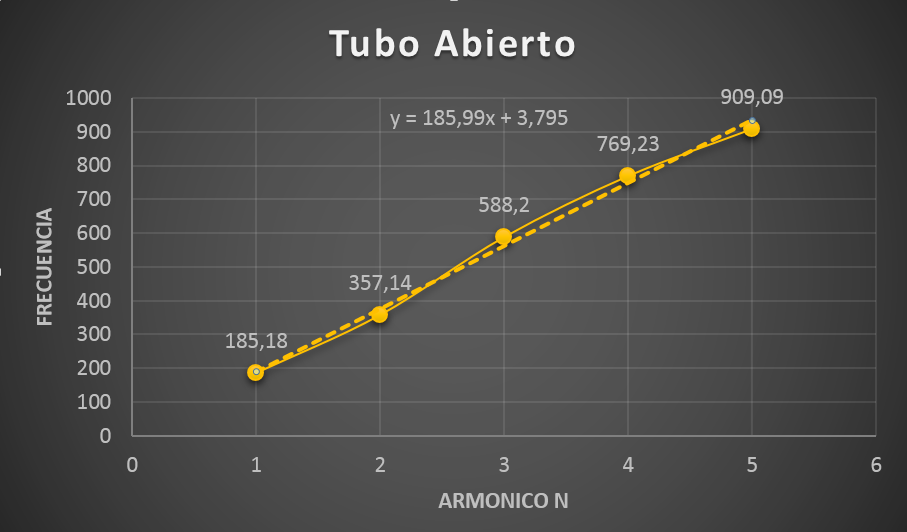
\includegraphics[width=0.85\textwidth]{tuboa}
  \caption{Representacion Grafica de los datos en Tubo \textbf{Abierto}.}
      \label{fig:pulsador}
\end{figure}
$$\\$$
\begin{figure}[H]
  \centering
     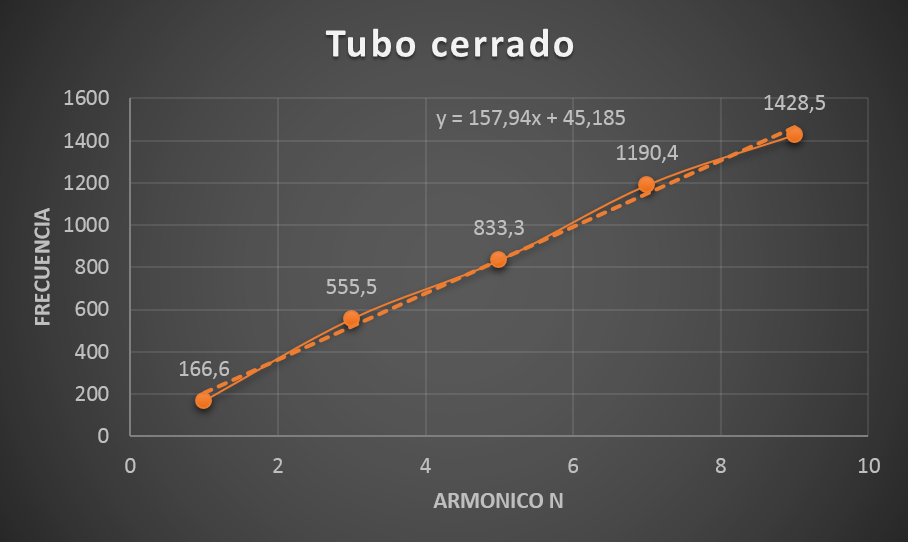
\includegraphics[width=0.85\textwidth]{tuboc}
  \caption{Representacion Grafica de los datos en Tubo \textbf{Cerrado}.}
      \label{fig:pulsador}
\end{figure}


Para \textbf{tubo abierto} Según la gráfica, la ecuación de la recta es$$f=185.99n+3.795$$La ecuación  teórica es $$f=\frac { n }{ 2*L } *v\quad ,\quad n=1,2,3$$Reemplazando$$\frac {n}{2*L}*v=185.99$$
$$\\$$
$$v=185.99*2*0.9$$
Como resultado obtenemos la velocidad del sonido en el aire:
$$v=334.77\frac{m}{s} $$
\textbf{Incertidumbre}
\begin{equation}
{ S }_{ m }={ S }_{ y }\sqrt { \frac { N }{ N\sum _{ i=1 }^{ n }{ { X }_{ i }^{ 2 } } -{ (\sum _{ i=1 }^{ n }{ { X }_{ i }^{ 2 } } ) }^{ 2 }\quad  }  }
\end{equation}

\begin{equation}
{ S }_{ y }=\sqrt { \frac { { \sum _{ i=1 }^{ n }{ { ({ y }_{ i }-{ m }x_{ i }-b) }^{ 2 } }  } }{ N-2\quad  }  } 
\end{equation}
Para \textbf{tubo abierto} tenemos :
$${ S }_{ y }=7.59498519$$
$$ U_{ E }=1.96*7.59=14.8794$$
$$v=(334.77_{ - }^{ + }\quad 14.88){ m }/{ s }$$
Para \textbf{tubo cerrado} tenemos  según la grafica la ecuacion de la recta es : $$f=157.9n+45.185$$La ecuacion teorica es:$$f=\frac { n }{ 4*L } v,\quad n=1,3,5\ldots$$Reemplazando
$$\frac { n }{ 4*L } v=157.9$$
$$\\$$
$$v=157.9*4*0.5$$
$$\\$$
Como resultado obtenemos la velocidad el sonido en el aire:
$$v=315.8\frac{ m }{ s } $$
Calculando la incertidumbre para tubo cerrado tenemos :
$${ S }_{ y }=2.92570279$$
$$ U_{ E }=1.96*2.92=5.7532$$
$$v=(315.8_{ - }^{ + }\quad 5.7532){ m }/{ s }$$
\subsection{(Pregunta 4.7.4)}
\textit{\textbf{4.} Promedie los resultados para la velocidad obtenida de los dos gráficos y obtenga el mejor estimado con su respectiva incertidumbre. }
$$vpromedio=\frac { 334,77+315.8 }{ 2 }$$
$$\\$$
$$vpromedio=325.285\frac { m }{ s } $$
\subsection{(Pregunta 4.7.5)}
\textit{\textbf{5.} Compare el valor obtenido con el calculado a través de la expresión $v =333.5 +0.607T$, donde  $T$ es la temperatura en grados Celsius medida en el laboratorio. Halle el porcentaje de error y explique las posibles razones de la discrepancia.}
$$v=333.5+0,607*T$$
La Temperatura del laboratorio es de $28^oC$. Reemplazando en la ecuación anterior tenemos:
$$v=333.5+(0,607)(28)$$
$$v=350.496\frac {m}{s} $$
Para representar el error porcentual entre el \emph{Valor experimental} y el \emph{Valor esperado} tomado en la medida se sigue la siguiente ecuación:
\begin{equation}
    \% Error = \frac{|Valor \ esperado-Valor \ experimental|}{Valor esperado}*100\%
\end{equation}
Donde el dato teórico será la velocidad del sonido teórica \textbf{V=340$\frac{m}{s}$} Y el dato experimental será la velocidad del sonido obtenida en este informe \textbf{V=350.496$\frac{m}{s}$}.
\begin{equation}
    \% Error = \frac{| 340 -350.496|}{340}*100\%
\end{equation}
Obteniendo el siguiente error porcentual:
\begin{equation}
    \% Error = 3.0897\%
\end{equation}
\textbf{Observación}: Lo que podemos observar en este punto es que se presenta un leve error porcentual dado que los factores climáticos del medio en el que se propagan las ondas pueden influenciar en la velocidad de propagación ( para este caso la velocidad de propagación del sonido ) ya que a mayor temperatura las partículas del medio se mueven mas rápido.
\subsection{Conclusiones }
De la practica experimental, y la teoría conocida podemos concluir:
\begin{itemize}
	\item  Confirmamos que los armónicos para tubos cerrados y tubos abiertos son difieren después de $n = 1$.
    \item Podemos también ver una especie de analogía entre las ondas estacionarias en una cuerda (laboratorio realizado anteriormente) con las ondas estacionarias en una columna de aire,  en ambos casos las ondas estacionarias se producen por la superposición de ondas longitudinales.
    \item Se demostró que es posible obtener mediante la toma de datos, la velocidad del sonido en el aire y también el efecto que tiene la temperatura sobre esta variable.
\end{itemize}
\section{Bibliografia}
$[1]$ Raymond A. Serway Physics for Scientists and Engineers with Modern Physics. 
$\\$
$[2]$ Sears and Zemansky's University Physics.
$\\$
$[3]$ Fishbane, Paul y otros. Física para ciencias e ingeniería, Volumen I. Prentice Hall, 2001.
$\\$
$[4]$ Serway, Taymond. Física Tomo I, Cuarta edición. McGraw Hill, 1997.
\end{document}